%%%%%%%%%%%%%%%%%%%%%%%%%%%%%%%%%%%%%%%%%%%%%%%%%%%%%%%%%%%%%%%%%%%%%%%%%%%%%%%
\documentclass{report}
\newcommand{\path}{../../../assets/settings}
\newcommand{\inputado}{solo para indicar a los importados que no incluyan las referencias}
\input{\path/newcommand.tex}
\input{\path/usepackage.tex}
% \input{../../../assets/settin

%%%%%%%%%%%%%%%%%%%%%%%%%%%%%%%%%%%%%%%%%%%%%%%%%%%%%%%%%%%%%%%%%%%%%%%%%%%%%%%
\title{\includegraphics[width=0.13\textwidth]{logo} \\ \proyectotitulo \\ \proyectosubtitulo }
\author{
\\
\vspace{2cm} \\
TITULAR: AYUNTAMIENTO DE MADRID \\
CIF: XXXXXXXX \\
EMPLAZAMIENTO INSTALACIÓN: CALLE GRAL. MOSCARDO, 2 \\
LOCALIDAD: MADRID - 29003  \\
\\
\vspace{2cm} \\
Proyectista: \proyectosubtitulo \\
INGENIERÍA: KGNETE, INGENIERÍA Y CONSULTORÍA S.L. \\
INGENIERÍA: KGNETE, INGENIERÍA Y CONSULTORÍA S.L. \\
N$^o$ Colegiado: 26975
\vspace{2cm} \\
}
\date{\today}
\begin{document}








\maketitle
\tableofcontents





\documentclass{article}

\input{../../../assets/settings/newcommand.tex}
\input{../../../assets/settings/usepackage.tex}
% \input{../../../assets/settings/quitarnumerossecciones.tex}

% \usepackage{nopageno} % Paquete para desactivar la numeración de páginas

\title{Memoria}
\author{KGNETE}
\date{\today}

\begin{document}

\maketitle

\chapter{Memoria}

\section{Objeto}
El objeto es justificar las soluciones adoptadas, su adecuación a la normativa legal aplicable y, conjuntamente
con los planos y el pliego de condiciones, describir de forma unívoca el objeto del Proyecto.

\section{Alcance}

Se genera la energia que se consume en la propia instalacion.

\section{Antecedentes}

Se trata de una ampliación de la instalacion receptora con una instalacion generadora de electricidad.

\section{Normas y referencias}

La instalación se realizará conforme a la normativa vigente, incluyendo pero no limitándose a:

\subsection{Disposiciones legales y normas aplicadas}

% \href{https://www.idae.es/sites/default/files/documentos/publicaciones_idae/2023_10_20_Guia_Autoconsumo_Ayuntamientos_v4.pdf}{Disposiciones legales y normas aplicadas}
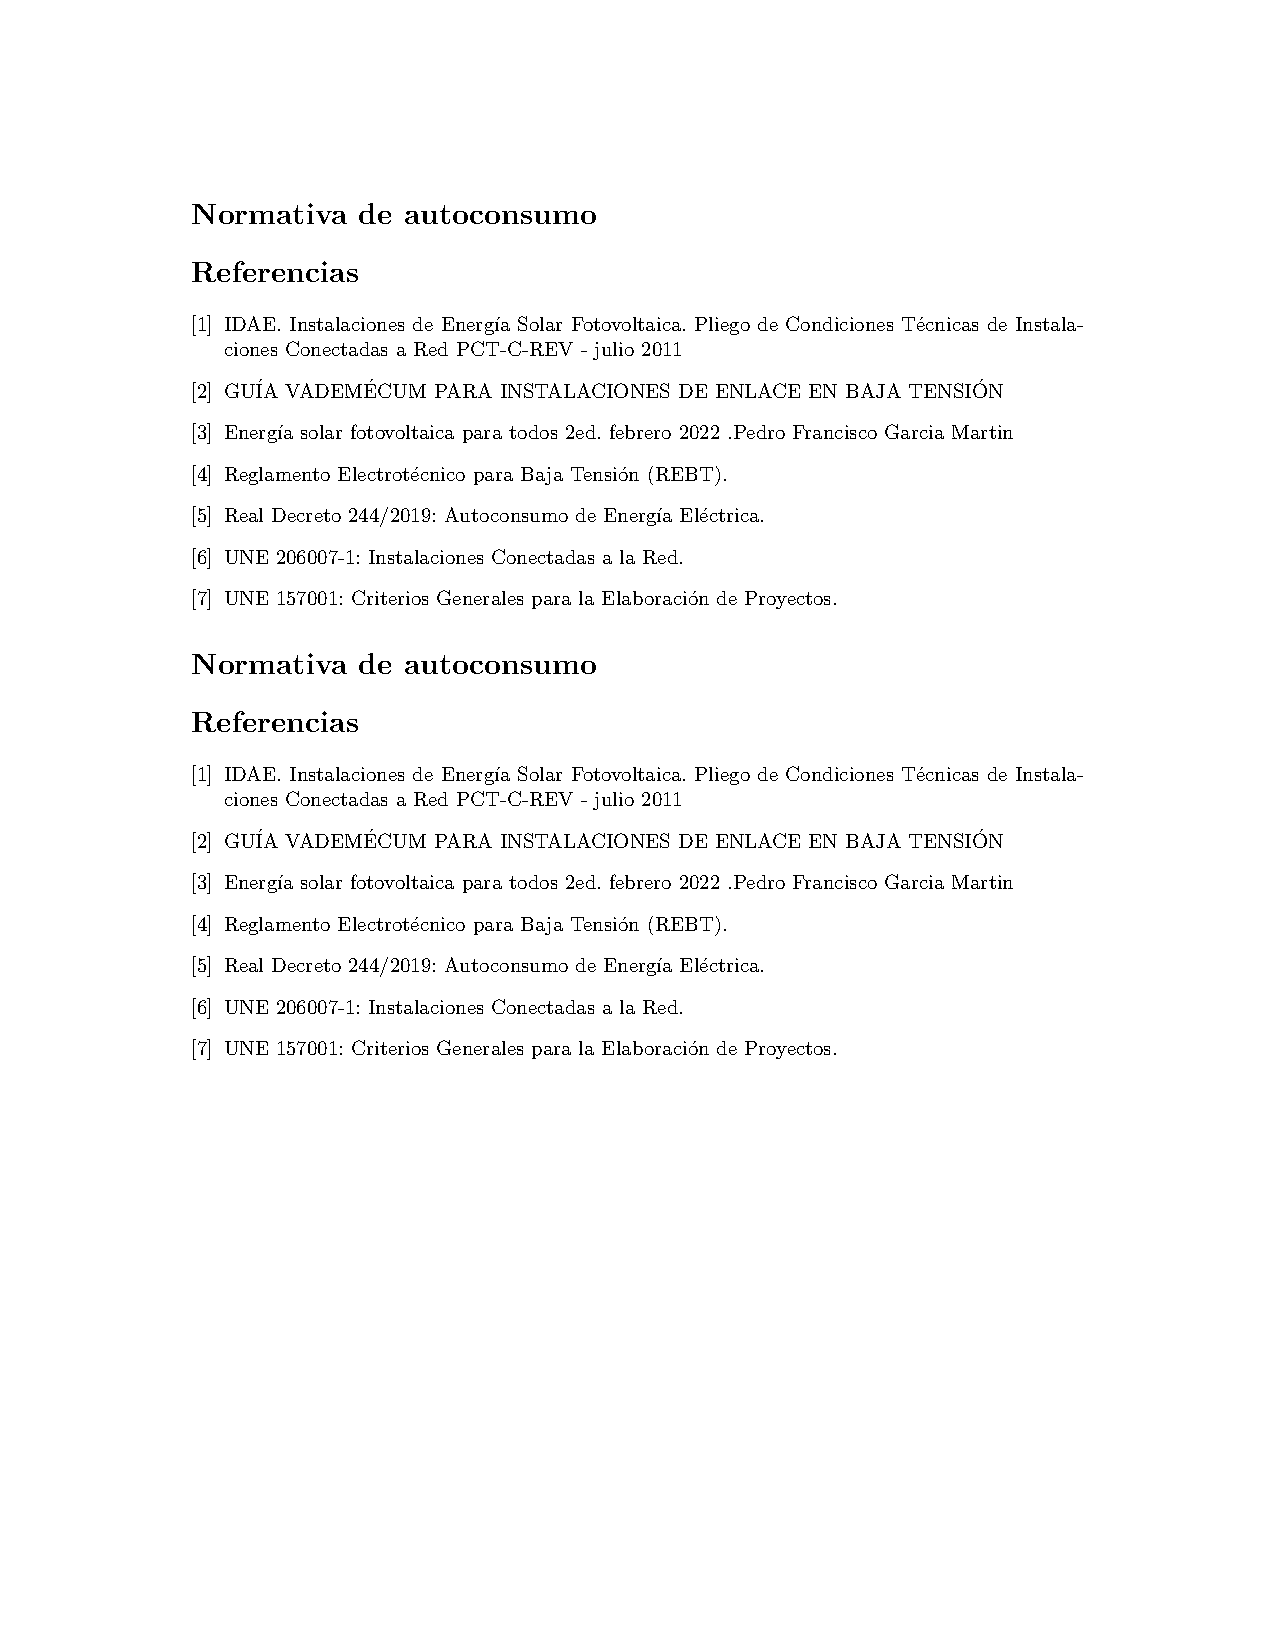
\includepdf[pages=-, pagecommand={\thispagestyle{fancy}}]{../DOCUMENTOS/Normativa Autoconsumo.pdf}


Las instalaciones de autoconsumo de cualquier tecnología de generación, están sometidas a la normativa eléctrica que les aplique en función de su potencia y de la conexión que realicen, bien en baja tensión (BT) o en alta tensión (AT).


En este apartado se describen los conceptos fundamentales extraídos de la normativa eléctrica y las principales autorizaciones que las instalaciones de autoconsumo deben obtener, puesto que dependen del tamaño de la instalación (en términos de potencia) y pueden servir de guía a los técnicos municipales para valorar su complejidad y la magnitud de las actuaciones que implican.

\subsubsection{Solicitud de acceso y conexión}

El acceso y conexión aparece regulado por el Real Decreto 1183/2020, de 29 de diciembre, de acceso y conexión a las redes de transporte y distribución de energía eléctrica.

El procedimiento a seguir queda regulado por el mismo Real Decreto y por la Circular 1/2021 de 20 de enero, de la Comisión Nacional de los Mercados y la Competencia, por la que se establece la metodología y condiciones del acceso y de la conexión a las redes de transporte y distribución de las instalaciones de producción de energía eléctrica.

Con este trámite, se solicita permiso para acceder a la red pública de transporte o distribución y se obtienen las condiciones en las que dicho acceso es posible y cómo y dónde deberá realizarse la conexión a la misma. Además, se obtienen la potencia que será posible conectar.

Este trámite incluye la presentación de garantías económicas por una cuantía equivalente a 40 €/kW de potencia que se solicita, y cuyo resguardo de presentación se deposita ante el órgano competente para otorgar la autorización de la instalación. La finalidad de la garantía será la obtención de la autorización de explotación.

Las instalaciones de autoconsumo SIN excedentes están exentas de realizar este trámite de acceso y conexión y, por tanto, tampoco tienen que presentar la garantía.

Las instalaciones de autoconsumo CON excedentes de potencia igual o inferior a 15 kW que se ubiquen en suelo urbanizado que cuente con las dotaciones y servicios requeridos por la legislación urbanística, también están exentas de realizar el trámite de acceso y conexión y por tanto tampoco deberán presentar la garantía.

El resto de instalaciones de autoconsumo CON excedentes siempre que sean de potencia igual o inferior a 100 kW, sí tendrán que realizar el trámite de acceso y conexión, pero no precisan aportar la garantía, salvo que estas instalaciones formen parte de una agrupación cuya potencia sea superior a 1 MW, de acuerdo con la definición de agrupación establecida en el artículo 7 del Real Decreto 413/2014, de 6 de junio. En el caso de que además sean de potencia inferior a 15kW podrán acogerse al procedimiento abreviado, cuyos plazos serían la mitad que en el procedimiento general.

Desde la aprobación del Real Decreto-ley 23/2020, de 23 de junio es posible que la potencia de acceso concedida sea inferior a la potencia que figura en la autorización administrativa. La capacidad de acceso será la potencia activa máxima que se le permite verter a la red a una instalación de generación de electricidad.

\subsubsection{Autorización administrativa}

La Ley 24/2013, de 26 de diciembre, del Sector Eléctrico regula el régimen de autorizaciones de las instalaciones de generación, incluidas las de autoconsumo, entre las que se incluyen:

- a) Autorización administrativa previa, que se tramitará con el anteproyecto de la instalación como documento técnico y, en su caso, conjuntamente con la evaluación de impacto ambiental, según lo dispuesto en la Ley 21/2013, de 9 de diciembre, de evaluación ambiental, y otorgará a la empresa autorizada el derecho a realizar una instalación concreta en determinadas condiciones.

- b) Autorización administrativa de construcción, que permite al titular realizar la construcción de la instalación cumpliendo los requisitos técnicos exigibles. Para solicitarla, el titular presentará un proyecto de ejecución junto con una declaración responsable que acredite el cumplimiento de la normativa que le sea de aplicación. La tramitación y resolución de autorizaciones definidas en los párrafos anteriores podrán efectuarse de manera consecutiva, coetánea o conjunta.

- c) Autorización de explotación, que permite, una vez ejecutado el proyecto, poner en tensión las instalaciones y proceder a su explotación.

El Real Decreto 1955/2000 en su artículo 111 exime de este trámite a las instalaciones de tensión inferior a 1kV. Adicionalmente, el Real Decreto 1699/2011 exime a las instalaciones de producción de energía eléctrica con potencia nominal no superior a 100 kW, conectadas directamente a una red de tensión no superior a 1 kV, ya sea de distribución o a la red interior de un consumidor.

\subsubsection{Reglamentos técnicos}

Ley 24/2013, de 26 de diciembre, del Sector Eléctrico, establece que las instalaciones de autoconsumo conectadas en baja tensión se ejecutarán de acuerdo con lo establecido en el Reglamento Electrotécnico de Baja Tensión (REBT) y sus Instrucciones Técnicas complementarias (ITC-BT). Según determina la ITC-BT-40, será admisible la conexión a BT de las instalaciones de  autoconsumo CON excedentes de hasta 100 kW y en todas las instalaciones de autoconsumo SIN excedentes.

Por esta razón, cualquier instalación de autoconsumo conectada a las redes de baja tensión contará con un Certificado de Instalación eléctrica (CIE) firmado por una empresa instaladora habilitada y debidamente diligenciado por el órgano competente de la comunidad autónoma, que asegurará que esta ha sido llevada a cabo en base a lo establecido en el REBT.

De acuerdo con el REBT, si la instalación tiene una potencia superior a 10 kW deberá disponer de un proyecto técnico firmado por técnico competente. Las instalaciones de menor potencia (hasta 10 kW) únicamente tienen obligación de disponer de una Memoria Técnica de Diseño (MTD) según el formato de la comunidad autónoma, firmada por la empresa instaladora habilitada.

En el caso de las instalaciones conectadas en alta tensión el reglamento aplicable será el Reglamento de Instalaciones Eléctricas de Alta Tensión (RAT) y sus Instrucciones Técnicas complementarias (ITC-RAT)

\subsubsection{Registro Administrativo de Autoconsumo (RADNE)}

El RD 244/2019 establece que todas las instalaciones de autoconsumo deberán estar registradas en el Registro Administrativo de Autoconsumo que es competencia de la Dirección General de Política Energética y Minas del Ministerio para la Transición Ecológica y el Reto Demográfico y que se encuentra regulado en el artículo 19 de dicho real decreto.

Las comunidades autónomas y las ciudades autónomas de Ceuta y Melilla pueden crear sus propios registros de autoconsumo de carácter autonómico, pero en cualquier caso deben proporcionar la información necesaria para la inscripción (descrita en el ANEXO II del RD 244/2019) al Ministerio.

Este paso administrativo es transparente para el consumidor y/o promotor de la instalación de autoconsumo ya que se realiza de oficio entre administraciones y resulta el último trámite en la legalización de una instalación de autoconsumo. Para obtener más información sobre la tramitación administrativa de las instalaciones de autoconsumo puede consultar la Guía Profesional de Tramitación del Autoconsumo disponible en <https://www.idae.es/>

\subsubsection{Ordenanzas urbanísticas}

\subsubsection{Autónomica}

Leyes de urbanismo y de ordenación del suelo.

\subsubsection{Municipal}

El municipio  establece tres tipos de trámites para estas autorizaciones:

- Licencia de obra.

- Declaración responsable de obra.
Normalmente se destina a aquellas actuaciones técnicamente sencillas y que no precisen
elementos estructurales, y que no supongan alteración del volumen, del uso principal de
las instalaciones y servicios de uso común o del número de viviendas y locales, ni afecten
a la composición exterior, a la estructura o a las condiciones de habitabilidad o seguridad.

- Comunicación previa a la ejecución de obra.
Normalmente pequeñas actuaciones y/o reformas.

La instalacion fotovoltaicas de autoconsumo se ubica en la cubierta de edificio ya existente, cumplen las características de sencillez técnica y no afectación a elementos estructurales del edificio. En ningún caso supone aumento de superficie habitable.

Estas características de las instalaciones de autoconsumo fotovoltaico sobre edificacion permite a los municipios la aplicación de procedimientos de declaración responsable o comunicación previa en la concesión de las licencias de obras.

Para la redacción del presente proyecto se han tenido en cuenta las normas y disposiciones legales (leyes, reglamentos, ordenanzas, nor-
mas de obligado cumplimiento por su inclusión en disposiciones legales, etc.)

% {excel2md.normativa()}


% \subsection{Programas de cálculo}

% - Excel

% - PHOTOVOLTAIC GEOGRAPHICAL INFORMATION SYSTEM (PVGIS)

% \subsection{Plan de gestión de la calidad aplicado durante la redacción del Proyecto}

% Los procesos específicos utilizados

% - Aseguramiento de la calidad del proceso
% Durante la ejecución del proyecto, se monitorean y evalúan continuamente los procesos para asegurarse de que se estén siguiendo según lo planeado. Esto implica revisar regularmente si se cumplen los estándares y realizar ajustes si es necesario.

% - Revisiones:
% Se llevan a cabo revisiones periódicas de las actividades y los productos entregables para identificar posibles problemas o desviaciones con respecto a los estándares de calidad establecidos.

% - Gestión de cambios:
% El control de cambios es esencial para asegurar la calidad. Cualquier cambio en los requisitos o en el alcance del proyecto debe ser gestionado cuidadosamente para evitar impactos negativos en la calidad

% - Pruebas y validación:
% Se realizan pruebas exhaustivas en todas las fases del proyecto para verificar que los productos cumplen con los requisitos y estándares de calidad establecidos. Esto puede incluir pruebas de funcionalidad, rendimiento, seguridad, entre otras.

% - Mejora continua:
% Después de la finalización del proyecto, se realiza una revisión exhaustiva para analizar lecciones aprendidas y identificar áreas de mejora. Esto alimenta el ciclo de mejora continua, permitiendo ajustes en los procesos para futuros proyectos.

% \subsection{Bibliografía}

% - Instalaciones solares fotovoltaicas 2ª edición , Miguel Moro Vallina, 21/2/2024

% - Configuración de instalaciones solares fotovoltaicas 2.ª edición 2022 , Julian Cantos Serrano, 7/7/2023
% % Para justificar las soluciones adoptadas en el Proyecto se han considerado de interes:

% % {o.Normativa{o.Normativa{'Tipo'} == 'Bibliografía'}.loc{:, 'Denominacion'}.dropna().reset_index(drop=True).to_markdown(headers={''*5})}

% \subsection{Otras referencias}

% - \href{https://www.idae.es/tecnologias/energias-renovables/oficina-de-autoconsumo/guias-tecnicas-sobre-autoconsumo}{Guías técnicas y Formación sobre autoconsumo,  IDAE}

% \section{ Definiciones y abreviaturas}

% % <!-- 
% % En este capítulo de la memoria se deben relacionar todas las definiciones, abreviaturas, etc. que se han utilizado y su significado. 
% % -->

% % {indice.abreviaturas()}

% \section{ Requisitos de diseño}

% <!-- 
% En este capítulo de la memoria se deben describir las bases y datos de partida que se derivan de:
%  el cliente,
%  el emplazamiento, y su entorno socio-económico y ambiental,
%  los estudios realizados encaminados a la definición de la solución adoptada,

%  las interfaces con otros sistemas o elementos externos al proyecto u otros que condicionan las soluciones técnicas del mismo.
%  -->

\section{ Análisis de soluciones}


\addcontentsline{toc}{subsection}{Disposicion de los paneles}
\includepdf[pages=-, pagecommand={\thispagestyle{fancy}}]{../ESTUDIOS/Disposicion de los paneles.pdf}


\addcontentsline{toc}{subsection}{Rentabilidad de una bateria}
\includepdf[pages=-, pagecommand={\thispagestyle{fancy}}]{../ESTUDIOS/Rentabilidad de una bateria.pdf}



\section{ Resultados Instalacion FV}

\addcontentsline{toc}{subsection}{Rentabilidad de una bateria}
\includepdf[pages=-, pagecommand={\thispagestyle{fancy}}]{../CALCULOS/Resultados Instalacion FV.pdf}



% - Las características definitorias de la instalación elegida, indicada enla tabla esta desarrolada en el apartado planos.

\subsection{Rendimiento de un sistema FV conectado a red (PVGIS)}
\includepdf{../../assets/varios/PVGIS.pdf}


\subsection{Analisis finaciero (SAM)}

\section{ Planificación}

En relación al proceso de materialización del Proyecto, se definen las etapas agrupadas segun la figura.

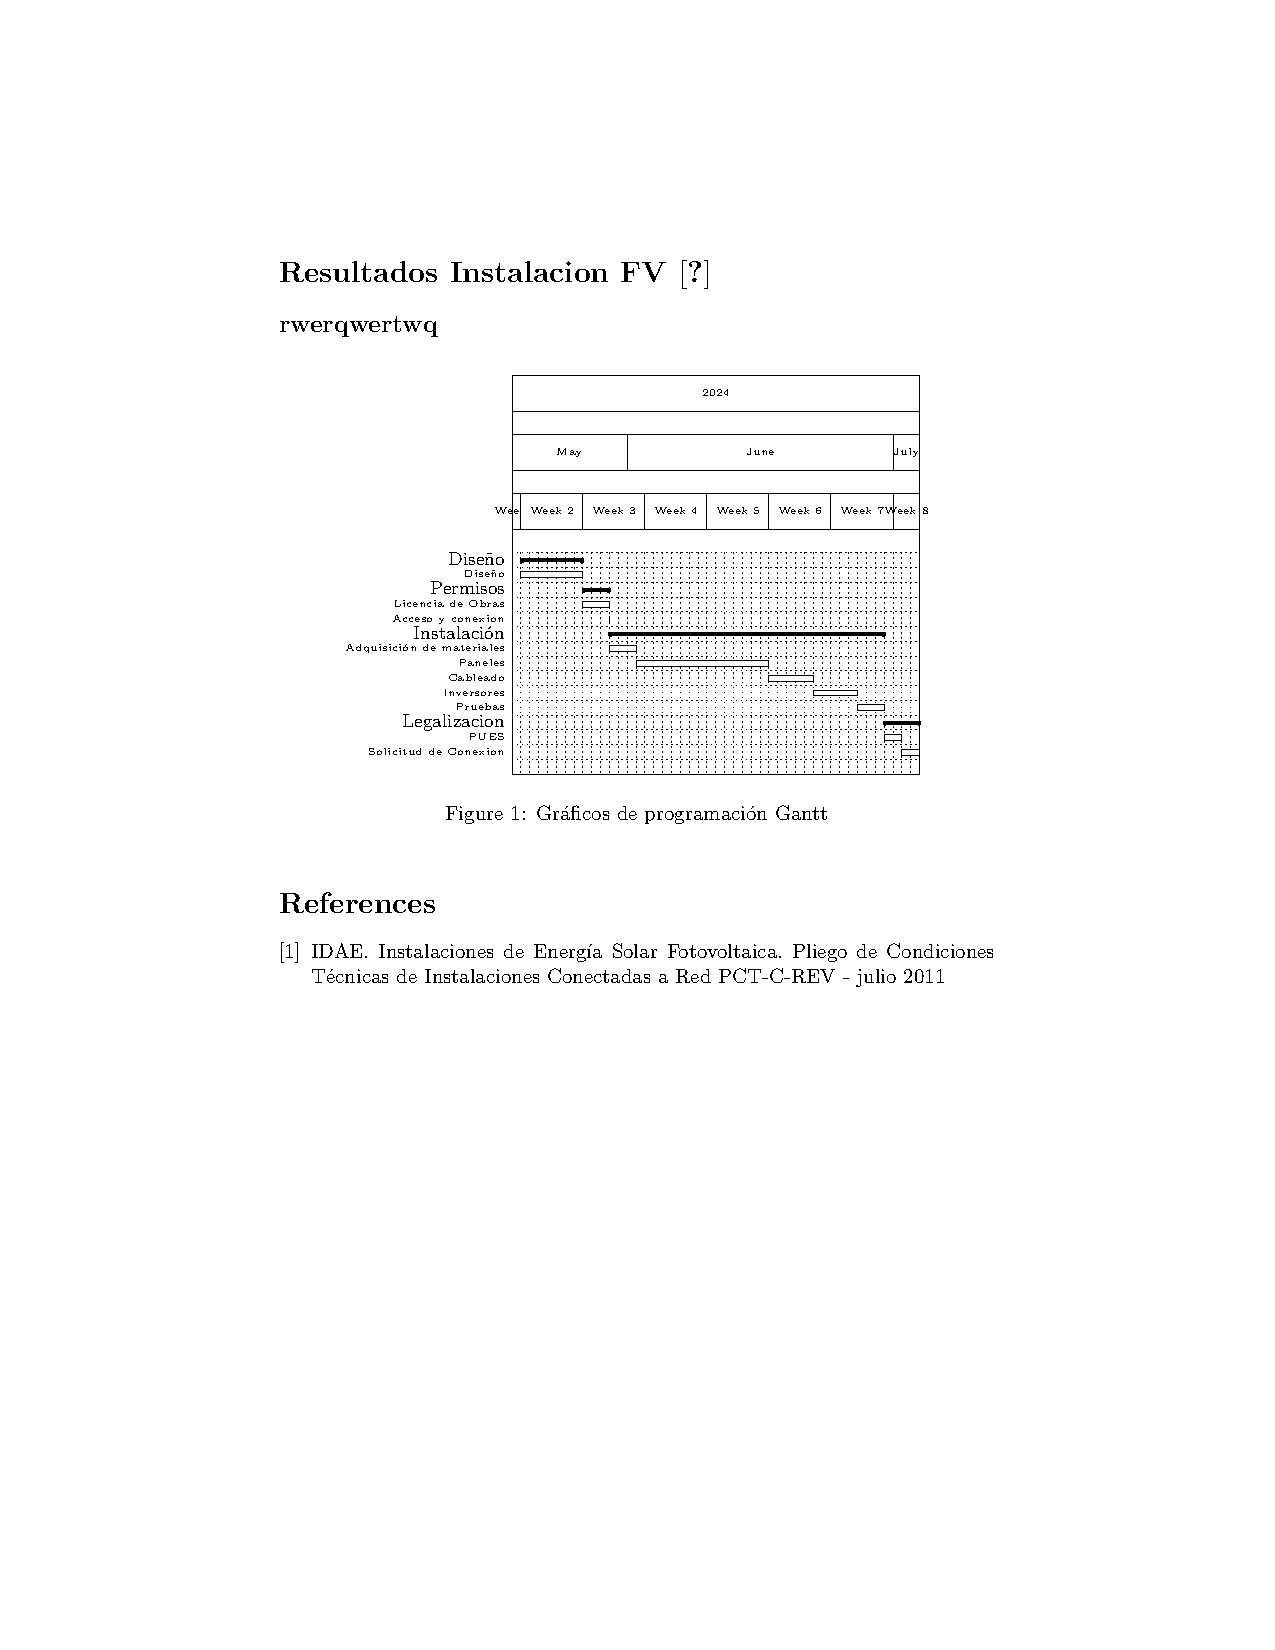
\includepdf[pages=-, pagecommand={\thispagestyle{fancy}}]{../DOCUMENTOS/Planificacion.pdf}

% {figltx.gantt()}

\section{ Orden de prioridad entre los documentos}

El orden de prioridad debe ser el siguiente:

1 Planos.

2 Pliego de condiciones.

3 Presupuesto.

4 Memoria.



\end{document}

\documentclass{article}
\newcommand{\path}{../../../assets/settings}
\newcommand{\inputado}{solo para indicar a los importados que no incluyan las referencias}
\input{\path/newcommand.tex}
\input{\path/usepackage.tex}
% \input{../../../assets/settings/quitarnumerossecciones.tex}
% \usepackage{nopageno} % Paquete para desactivar la numeración de páginas
\title{ANEXOS}
\author{KGNETE}
\date{\today}
\begin{document}
\maketitle
\chapter{ANEXOS}
%%%%%%%%%%%%%%%%%%%%%%%%%%%%%%%%%%%%%%%%%%%%%%%%%%%%%%%%%%%%%%%%%%%%%%%%%%%%%%%
\section{Documentación de partida.}
%%%%%%%%%%%%%%%%%%%%%%%%%%%%%%%%%%%%%%%%%%%%%%%%%%%%%%%%%%%%%%%%%%%%%%%%%%%%%%%

%%%%%%%%%%%%%%%%%%%%%%%%%%%%%%%%%%%%%%%%%%%%%%%%%%%%%%%%%%%%%%%%%%%%%%%%%%%%%%%
\section{Cálculos.}
% %%%%%%%%%%%%%%%%%%%%%%%%%%%%%%%%%%%%%%%%%%%%%%%%%%%%%%%%%%%%%%%%%%%%%%%%%%%%%%%
% \addcontentsline{toc}{subsection}{Diseno campo fotovoltaico}
% \includepdf[pages=-, pagecommand={\thispagestyle{fancy}}]{../CALCULOS/Diseno del generador.pdf}
\input{../CALCULOS/Diseno del generador}
\newpage
\input{../CALCULOS/Distancia minima entre filas de modulos}
\newpage
\input{../CALCULOS/Perdidas por orientacion e inclinacion}
\newpage
\input{../CALCULOS/Resultados Instalacion FV}
\newpage
\input{../CALCULOS/Análisis de seguridad estructural de las cubiertas}
\newpage

%%%%%%%%%%%%%%%%%%%%%%%%%%%%%%%%%%%%%%%%%%%%%%%%%%%%%%%%%%%%%%%%%%%%%%%%%%%%%%%


% %%%%%%%%%%%%%%%%%%%%%%%%%%%%%%%%%%%%%%%%%%%%%%%%%%%%%%%%%%%%%%%%%%%%%%%%%%%%%%%
\section{Anexos de aplicación}
% %%%%%%%%%%%%%%%%%%%%%%%%%%%%%%%%%%%%%%%%%%%%%%%%%%%%%%%%%%%%%%%%%%%%%%%%%%%%%%%
\subsection{Seguridad}
\subsection{Medio ambiente}
\subsection{Eficiencia energética.}
\subsection{Emplazamiento del proyecto,}
\subsection{Gestion de residuos}
\subsection{Certificaciones de solidez y Estudios de cargas}
% %%%%%%%%%%%%%%%%%%%%%%%%%%%%%%%%%%%%%%%%%%%%%%%%%%%%%%%%%%%%%%%%%%%%%%%%%%%%%%%


% %%%%%%%%%%%%%%%%%%%%%%%%%%%%%%%%%%%%%%%%%%%%%%%%%%%%%%%%%%%%%%%%%%%%%%%%%%%%%%%
\section{Estudios con entidad propia}

% %%%%%%%%%%%%%%%%%%%%%%%%%%%%%%%%%%%%%%%%%%%%%%%%%%%%%%%%%%%%%%%%%%%%%%%%%%%%%%%
\subsection{Estudio Basico de Seguridad}
\subsection{Estudio de Impacto Ambiental.}
% %%%%%%%%%%%%%%%%%%%%%%%%%%%%%%%%%%%%%%%%%%%%%%%%%%%%%%%%%%%%%%%%%%%%%%%%%%%%%%%


% %%%%%%%%%%%%%%%%%%%%%%%%%%%%%%%%%%%%%%%%%%%%%%%%%%%%%%%%%%%%%%%%%%%%%%%%%%%%%%%
%%%%%%%%%%%%%%%%%%%%%%%%%%%%%%%%%%%%%%%%%%%%%%%%%%%%%%%%%%%%%%%%%%%%%%%%%%%%%%%
% \subsubsection{PROTECCIONES CC}
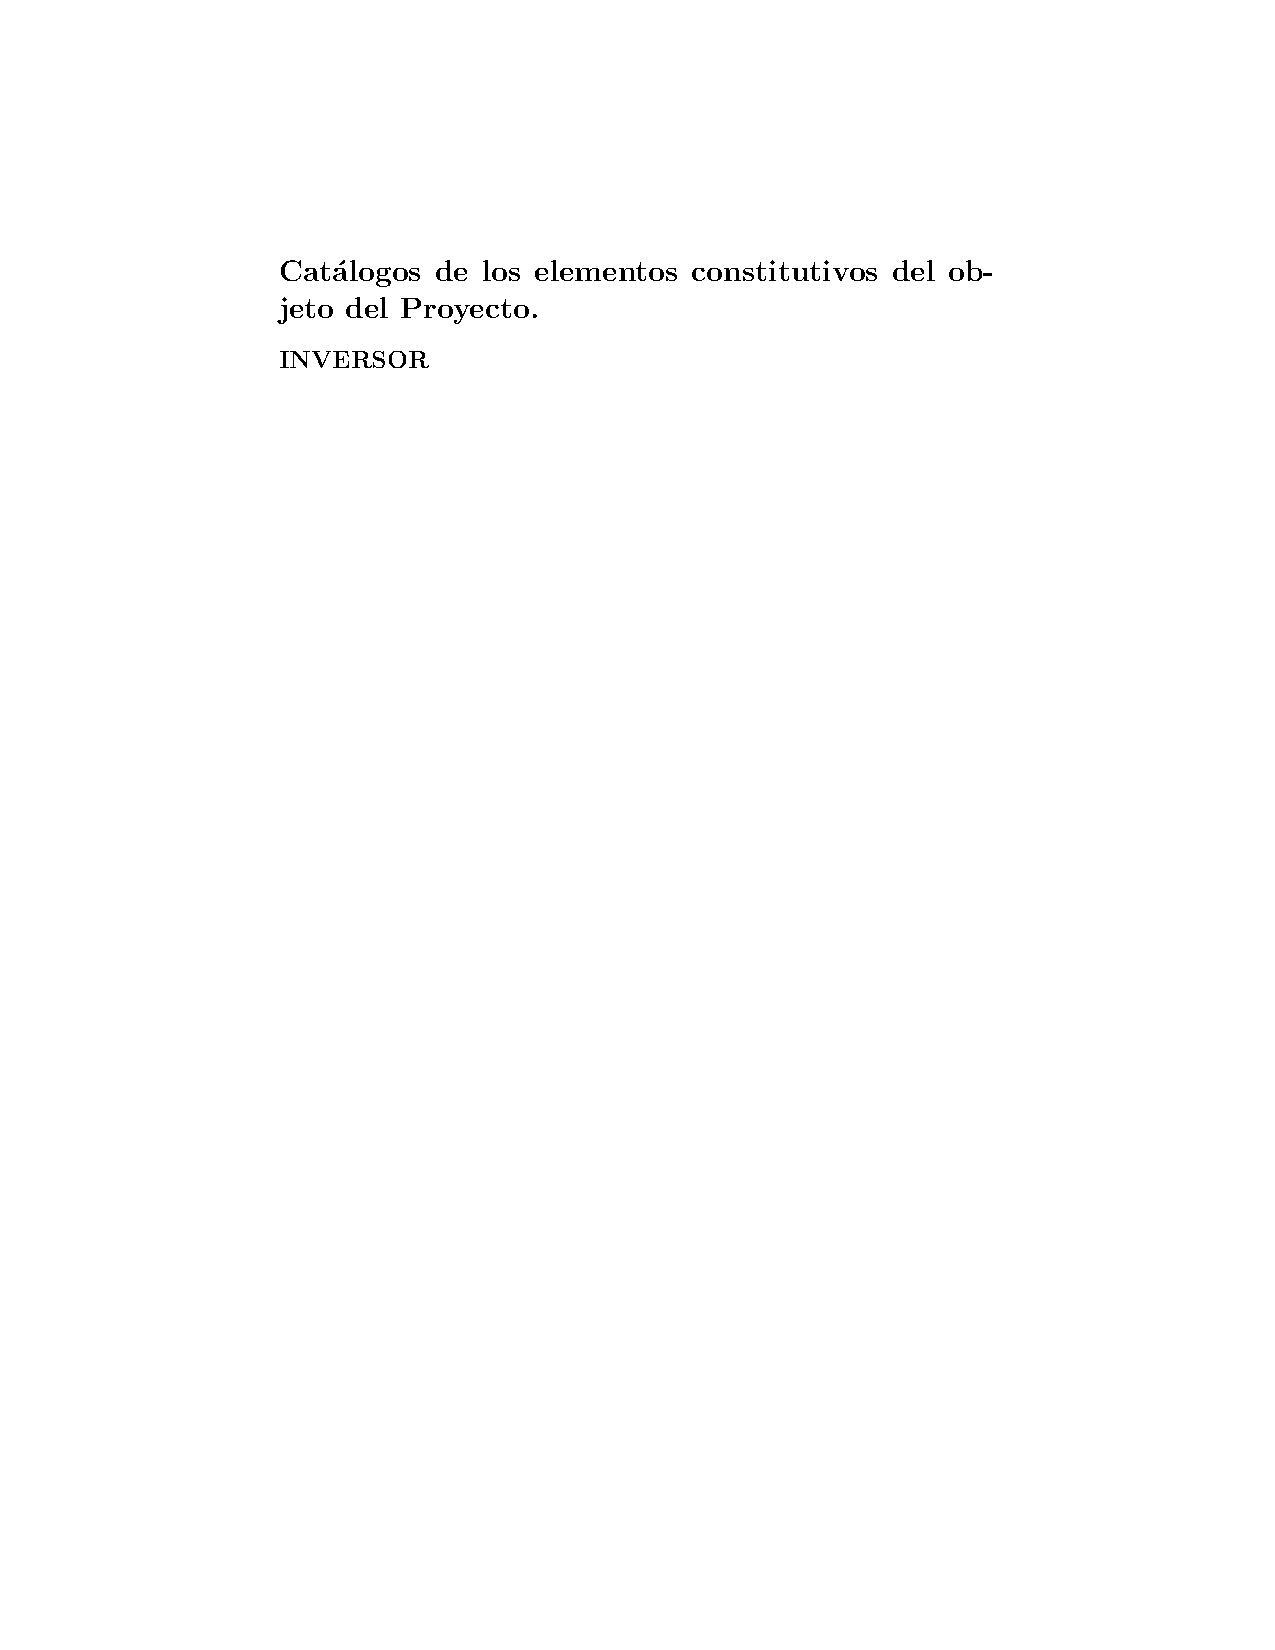
\includepdf[pages=-, pagecommand={\thispagestyle{fancy}}]{../DOCUMENTOS/Fichas Tecnicas.pdf}
% \subsubsection{PROTECCIONES AC}
% \includepdf[pages=-]{pdf/fichatecnica/inversor_protecciones.pdf}
%%%%%%%%%%%%%%%%%%%%%%%%%%%%%%%%%%%%%%%%%%%%%%%%%%%%%%%%%%%%%%%%%%%%%%%%%%%%%%%

\bibliographystyle{plainnat}
\bibliography{\path/referencias}


\end{document}





% %%%%%%%%%%%%%%%%%%%%%%%%%%%%%%%%%%%%%%%%%%%%%%%%%%%%%%%%%%%%%%%%%%%%%%%%%%%%%%%
\documentclass{article}
\input{../../../assets/settings/newcommand.tex}
\input{../../../assets/settings/usepackage.tex}
\usepackage{nopageno} % Paquete para desactivar la numeración de páginas

\begin{document}

\chapter{ PLIEGO DE CONDICIONES}
% copiado de algun otro prouecto
\section{ Descripción de las instalaciones}
Instalación fotovoltaica

% ```py
% <<o.v.loc['instalacion_tipo','v']>>
% para uso <<o.v.loc['instalacion_uso','v']>>
% situada en <<o.Ubicacion['v'].Direccion>>.
% Con potencia pico de <<o.v.loc['Np','v']*o.g['v'].Pmp/1000>> kW
% Esta compuesta por <<o.v.loc['Np','v']>> paneles de <<o.g['v'].Pmp>> W
% Se prevee que genere <<o.v.loc['Ep','v']>> kWh., 
% con un precio de la electicidad e IPC similar al ano anteior
% ahorro mensual del <<o.v.loc['Am','v']>> %
% periodo de amortizacion de <<o.v.loc['Pa','v']>> años.
% ```

\section{ Especificaciones de los materiales y elementos constitutivos}


\subsection{PlacaFV}
\PlacaFV

\subsection{Soporte}
\Soporte

\subsection{Inversor}
\Inversor

\subsection{Bateria}
\Bateria

\subsection{Cable}
\Cable
Los cables cumplirán con las características especificadas la memoria y planos. Todos ellos serán de marca reconocida en el mercado y cumplirán las normas del REBT así como las normas UNE correspondientes. El material eléctrico será seleccionado de modo que se asegure que su temperatura máxima superficial no exceda la temperatura de ignición de los gases, vapores, polvos o fibras que puedan presentarse. Los materiales eléctricos estarán protegidos contra las influencias externas. Las exigencias de construcción asegurarán la conservación del modo de protección cuando el material se utilice en las condiciones específicas de servicio. El material eléctrico será utilizado en la gama de temperaturas para la que se ha diseñado y que deberá incluirse en su marcado. Si no se da ninguna referencia se considera que el margen de utilización está comprendido entre  -20oC y 40oC. Otras temperaturas deberán indicarse expresamente en el certificado del laboratorio.


\subsubsection{ CABLES CONDUCTORES}

Todos los conductores empleados en la instalación serán de cobre (salvo indicación especial) y deberán cumplir la norma UNE-2003, UNE-21022 o UNE-21064.

Su aislamiento será de polietileno reticulado y cubierta exterior de PVC, apto para una tensión de servicio de 0.6/1 Kv. y 4 Kv. de tensión de prueba. La designación UNE de los mismos es RV-0.6/1KV.

Los conductores de secciones comprendidas entre 1 y 4 mm2  serán como mínimo de clase 1. Los conductores de 6 mm y más serán como mínimo de clase 2.

Las entradas de los cables y de los tubos a los aparatos eléctricos se realizará de acuerdo con el modo de protección  previsto.

Los orificios del material eléctrico para entradas de cable o tubos no utilizados deberán cerrarse mediante piezas acorde con el modo de protección de que vaya dotado dicho material.

En caso necesario, los cables y tubos estarán sellados para evitar el paso de gases y líquidos.

El tipo de cable será el especificado en la memoria y planos. Se instalarán cortafuegos para evitar el corrimiento de gases, vapores y llamas por el interior de los tubos.

Todo conductor debe poder seccionarse, en cualquier punto de la instalación en que derive, utilizando un dispositivo apropiado, tal como un borne de conexión, de forma que permita la separación completa de cada circuito derivado del resto de la instalación.

Para el tendido de conductores la temperatura ambiente será superior a 10ºC, de no ser así se tomarán las precauciones establecidas por el fabricante.

\subsubsection{ CANALIZACIONES}

En el caso de proximidad de canalizaciones eléctricas con otras no eléctricas, se dispondrán de forma que entre las superficies exteriores de ambas se mantenga una distancia de, por lo menos, 3 cm. En caso de proximidad con conductos de calefacción, de aire caliente o de humo, las canalizaciones eléctricas se establecerán de forma que no puedan alcanzar una temperatura peligrosa y, por consiguiente, se mantendrán separadas por una distancia conveniente o por medio de pantallas calorífugas.

Las canalizaciones eléctricas no se situarán paralelamente por debajo de otras que puedan dar lugar a condensaciones, a menos que se tomen las disposiciones necesarias para proteger las canalizaciones eléctricas contra los efectos de las condensaciones.

Las canalizaciones eléctricas se dispondrán de modo que en cualquier momento se pueda controlar su aislamiento, localizar y separar las partes averiadas y, llegando el caso, reemplazar fácilmente los conductores deteriorados.

Las canalizaciones eléctricas se establecerán de forma que por conveniente identificación de sus circuitos y elementos se pueda proceder en todo momento a reparaciones, transformaciones, etc.

\subsubsection{ EMPALMES Y CONEXIONES}

Los empalmes y conexiones de los conductores subterráneos, se efectuará, siguiendo métodos o sistemas que garanticen una perfecta continuidad del conductor y del  instalador

\section{ Ejecución de las obras, productos, instalaciones o servicios}

En relación al proceso de materialización del Proyecto, se definen las etapas agrupadas segun la figura,con una duracion de {o.gantt['Duracion'].sum()} dias, se prevee la entrega  para el
{(date.today()+ timedelta(days=-7+int(o.gantt['Duracion'].sum()))).strftime("%d-%m-%Y")}

{figltx.gantt()}

\section{ Reglamentación y  normativa aplicables}
Para la redacción del presente proyecto se han tenido en cuenta las normas y disposiciones legales (leyes, reglamentos, ordenanzas, nor-
mas de obligado cumplimiento por su inclusión en disposiciones legales, etc.)

{excel2md.normativa()}

\section{ Otros Aspectos del contrato}

\subsubsection{ NATURALEZA}

Las condiciones técnicas que se detallan en este Pliego de  Condiciones Generales, complementan las mencionadas en las  especificaciones de la memoria, Planos y Presupuesto, que tienen, a todos  los efectos, valor de Pliego de Prescripciones Técnicas. Cualquier  discrepancia entre los diversos contenidos de los diferentes documentos  aludidos, será inmediatamente puesta en conocimiento de la Dirección  Facultativa de las Obras, única autorizada para su resolución.  

No obstante, en condiciones puntuales que pudieran existir entre los  distintos documentos, prevalecerá aquel que, según criterio de la Dirección  Facultativa, sea más favorable para la buena marcha de la ejecución de la  obra, teniendo en cuenta para ello la calidad e idoneidad de los materiales  y resistencia de los mismos, así como una mayor tecnología aplicable.  

Las obras objeto del contrato son las que quedan especificadas en los  restantes documentos que forman el proyecto, Memoria, Mediciones,  Presupuesto y Planos.  

\subsubsection{ CONDICIONES DE INDOLE FACULTATIVA}
\subsubsection{CONDICIONES GENERALES}

Previamente a la formalización del Contrato, el Contratista deberá   haber visitado y examinado el emplazamiento de las obras, y de sus  alrededores, y se habrá  asegurado que las características del lugar, su  climatología, medios de acceso, vías de comunicación, instalaciones  existentes, etc., no afectarán al cumplimiento de sus obligaciones  contractuales.  

Durante el período de preparación tras la firma del Contrato, deberá   comunicar a la Dirección de obra, y antes del comienzo de ésta: Los detalles  complementarios, la memoria de organización de obra, y el calendario de  ejecución pormenorizado.  

Para realizar las acometidas de la obra, o de la edificación, se deberá  de cumplir el reglamento de Baja Tensión y el Reglamento de Alta Tensión en  el caso de las instalaciones eléctricas. En las restantes instalaciones se cumplirán las Normas propias de cada Compañía de Servicios y de forma general las Normas Básicas correspondientes.

El Contratista, viene obligado a conocer, cumplir y hacer cumplir toda la normativa referente a la Seguridad y Salud de las Obras de Construcción,  instalando  todos los servicios higiénicos que sean precisos para el personal que intervenga en las obras.

Los operarios serán de aptitud reconocida y experimentados en sus respectivos oficios, actuando bajo las ordenes del encargado, siendo este el que vigile la obra y haga cumplir en todo momento el Real decreto 1627/97 sobre Seguridad y salud en la construcción.

La Dirección Facultativa podrá recusar a uno o a varios productores de la empresa o subcontratista de la misma por considerarlos incapaces, siendo obligación del Contratista reemplazar a estos productores o subcontratistas, por otros de probada capacidad.

El Contratista, por sí mismo o por medio de un jefe de obra, o del encargado, estará en la obra durante la jornada legal del trabajo, y acompañará a la Dirección Facultativa en las visitas que esta haga a la obra.

El contratista está obligado a realizar con su personal y materiales cuanto la dirección facultativa disponga para apeos, derribos, recalces o cualquier otra obra de carácter urgente, anticipando de momento este servicio.

Es obligación del contratista el ejecutar cuanto sea necesario para la buena construcción y aspecto de las obras, aún cuando no se halle expresamente estipulado en los documentos del Proyecto, y dentro de los límites de posibilidades que los presupuestos determinen para cada unidad de obra y tipo de ejecución.

Cualquier variación que se pretendiere ejecutar sobre la obra proyectada, deberá ser puesta en conocimiento del Ingeniero técnico director, y no podrá ser ejecutada sin su consentimiento. En caso contrario la Contrata, ejecutante de dicha unidad de obra, responderá de las consecuencias que ello originase. No será justificante ni eximente a estos efectos el hecho de que la indicación de la variación proviniera del señor Propietario.

\subsubsection{NORMALIZACION DE LA EMPRESA SUMINISTRADORA DE ENERGIA ELECTRICA}

El instalador está obligado a mantener el debido contacto con la empresa suministradora a través del Técnico Director de las instalaciones, para evitar criterios dispares así como para seguir las normas que dicte la Compañía.

\subsubsection{CONDICION FINAL}

La orden de comienzo de la obra será indicada por el Promotor o
Propietario, quien responderá de ello si no dispone de los permisos
correspondientes.



% \chapter{ PLIEGO DE CONDICIONES}
% % secciones segun la norma
% \minitoc

% % El pliego de condiciones es uno de los documentos que constituyen el Proyecto y tiene como misión establecer las con-
% % diciones técnicas, económicas, administrativas, facultativas y legales para que el objeto del Proyecto pueda

% % materializarse en las condiciones especificadas, evitando posibles interpretaciones diferentes de las deseadas.
% % Su contenido y extensión queda a criterio de su autor y en función del tipo de Proyecto.
% % En el caso de proyectos administrativos es suficiente con establecer las condiciones técnicas.

% \section{ Descripción de las obras, productos, instalaciones o servicios.}

% \section{ Las especificaciones de los materiales y elementos constitutivos del objeto del Proyecto}

% \subsubsection{ Listado completo de los mismos}

% \subsubsection{ Calidades mínimas a exigir para cada uno de los elementos constitutivos del Proyecto, indicando la norma (siexiste) que contemple el material solicitado,}
% \subsubsection{ las pruebas y ensayos a que deben someterse}

% \subsubsection{ Norma según la cual se van a realizar}

% \subsubsection{ las condiciones de realización}

% \subsubsection{ los resultados mínimos a obtener.}

% \section{ Ejecución de las obras, productos, instalaciones o servicios.}

% \section{ La reglamentación y la normativa aplicables incluyendo las recomendaciones o normas de no obligado cumplimiento que, sin ser preceptivas, se consideran de necesaria aplicación al Proyecto a criterio de su autor.}
% \section{ Aspectos del contrato que se refieran directamente al Proyecto y que pudieran afectar a su objeto}

% \subsubsection{ Documentos base para la contratación de su materialización.}

% \subsubsection{ Limitaciones en los suministros, }
% que especifiquen claramente dónde empieza y dónde termina la responsabilidad del
% suministro y montaje.

% \subsubsection{ Criterios de medición, valoración y abono.}

% \subsubsection{ Criterios para las modificaciones al proyecto original, }
% especificando el procedimiento a seguir para las mismas, su aceptación y cómo deben quedar reflejadas en la documentación final.

% \subsubsection{ Pruebas y ensayos, }
% especificando cuales y en qué condiciones deben someterse los suministros según lo indicado en el apartado b).

% \subsubsection{ Garantía de los suministros, }
% indicando el alcance, duración y limitaciones.

% \subsubsection{ Garantía de funcionamiento}


% %%%%%%%%%%%%%%%%%%%%%%%%%%%%%%%%%%%%%%%%%%%%%%%%%%%%%%%%%%%%%%%%%%%%%%%%%%%%%%%%%%%%%%%%%%%%%%%%%%%%%%%%%%%%%%%%%%%%%%%%%%%%%%%%%%%%%%%%%%%%%%%%%%%%%%%%%%%%%%%%%%%%%%%%%%%%%%%%%%
% %%%%%%%%%%%%%%%%%%%%%%%%%%%%%%%%%%%%%%%%%%%%%%%%%%%%%%%%%%%%%%%%%%%%%%%%%%%%%%%%%%%%%%%%%%%%%%%%%%%%%%%%%%%%%%%%%%%%%%%%%%%%%%%%%%%%%%%%%%%%%%%%%%%%%%%%%%%%%%%%%%%%%%%%%%%%%%%%%%
% %%%%%%%%%%%%%%%%%%%%%%%%%%%%%%%%%%%%%%%%%%%%%%%%%%%%%%%%%%%%%%%%%%%%%%%%%%%%%%%%%%%%%%%%%%%%%%%%%%%%%%%%%%%%%%%%%%%%%%%%%%%%%%%%%%%%%%%%%%%%%%%%%%%%%%%%%%%%%%%%%%%%%%
% %%%%%%%%%%%%%%%%%%%%%%%%%%%%%%%%%%%%%%%%%%%%%%%%%%%%%%%%%%%%%%%%%%%%%%%%%%%%%%%%%%%%%%%%%%%%%%%%%%%%%%%%%%%%%%%%%%%%%%%%%%%%%%%%%%%%%%%%%%%%%%%%%%%%%%%%%%%%%%%%%%%%%%%%%%%%%%%%%%

\end{document}

\documentclass{article}

\input{../../../assets/settings/newcommand.tex}
\input{../../../assets/settings/usepackage.tex}
% \input{../../../assets/settings/quitarnumerossecciones.tex}

% \usepackage{nopageno} % Paquete para desactivar la numeración de páginas

\title{PLIEGO DE CONDICIONES}
\author{KGNETE}
\date{\today}

\begin{document}

\maketitle
\section{PLIEGO DE CONDICIONES}

\subsection{CARECTERÍSTICAS DE LA EMPRESA INSTALADORA}
Las instalaciones eléctricas de baja tensión serán ejecutadas por la empresa instaladora
autorizada, contando para ello con instalador Autorizado en Baja Tensión, autorizado para el
ejercicio de la actividad según lo establecido en la correspondiente Instrucción Técnica
Complementaria del R.E.B.T., sin perjuicio de su posible proyecto y dirección de obra por
técnicos titulados pertenecientes a dicha empresa instaladora.




\subsection{CALIDAD DE LOS MATERIALES}
Todos los materiales a emplear en la presente instalación serán de primera calidad y reunirán
las condiciones exigidas en el Reglamento Electrotécnico para Baja Tensión y demás
disposiciones vigentes referentes a materiales y prototipos de construcción.
Todos los trabajos incluidos en el presente proyecto se ejecutarán con arreglo a las buenas
prácticas de las instalaciones eléctricas, de acuerdo con el Reglamento Electrotécnico para
Baja Tensión, y cumpliendo estrictamente las instrucciones recibidas por la Dirección
Facultativa, no pudiendo, por tanto, servir de pretexto al contratista la baja en subasta, para
variar esa esmerada ejecución ni la primerísimo calidad de las instalaciones proyectadas en
cuanto a sus materiales y mano de obra, ni pretender proyectos adicionales.
Es por ello que los elementos que se describen como posibles materiales a utilizar cumplen los
mínimos exigidos por los indicados en el proyecto. Si por motivos se utilizasen equipos
diferentes en la instalación, estos tendrían que ser de características equivalentes por las
indicadas en las fichas adjuntas en el anexo de equipos y calidades iguales o superiores.




\subsubsection{CONDUCTORES ELÉCTRICOS}
Los conductores utilizados se regirán por las especificaciones del proyecto, según se indica en
Memoria, Planos y Presupuesto.

El tipo de cable que se empleará será RV-K 0,6/1 kV, cuyas características técnicas son las que
se muestran a continuación:

Flama: No propagador de llama, UNE-20432.1 (IEC-332.1)

Conductor de Cu: Clase 5

Aislamiento: XLPE

Cubierta:
PVC

Temperatura máxima de utilización: 90 °C

Características constructivas: UNE-21 123 (P-2)

Los conductores de sección igual o superior a 6 mm² deberán estar constituidos por cable
obtenido por trenzado de hilo de cobre del diámetro correspondiente a la sección del conductor
de que se trate.

Para la selección de la sección de los conductores activos del cable adecuado a cada carga se
usará el más desfavorable entre los siguientes criterios:

- Intensidad máxima admisible. Como intensidad se tomará la propia de cada generador
fotovoltaico, partiendo de las intensidades nominales así establecidas, se elegirá la sección del
cable que admita esa intensidad de acuerdo a las prescripciones del Reglamento
Electrotécnico para Baja Tensión ITC-BT-19 o las recomendaciones del fabricante, adoptando
los oportunos coeficientes correctores según las condiciones de la instalación.

- Caída de tensión en servicio. La sección de los conductores a utilizar se determinará de forma
que la caída de tensión para la parte de continua no podrá ser superior al 1.5% y para la parte de
alterna no podrá ser superior al 1.5%.

La sección del conductor neutro será la especificada en la Instrucción ITC-BT-07, apartado 1,
en función de la sección de los conductores de fase o polares de la instalación.




\subsubsection{CONDUCTORES DE PROTECCIÓN}
Los conductores de protección serán del mismo tipo que los conductores activos
especificados en el apartado anterior, y tendrán una sección mínima a la fijada en la tabla 2 de
la ITC-BT-18, en función de la sección de los conductores de fase o polares de la instalación. Se
podrán instalar por las mismas canalizaciones que estos o bien en forma independiente.


\subsubsection{IDENTIFICACIÓN DE LOS CONDUCTORES}
Para la identificación de los conductores en la parte de corriente continua se marcarán de
forma permanente el positivo de color Rojo y el negativo de color Azul, los colores de los
recubrimientos serán Azul para el neutro, Marrón, Gris o Negro para las fases y Amarillo-Verde
para los de protección.

Las canalizaciones eléctricas se establecerán de forma que por conveniente identificación de
sus circuitos y elementos, se pueda proceder en todo momento a reparaciones,
transformaciones, etc.



\subsubsection{CANALIZACIONES}
Las características de protección de la unión entre el tubo y sus accesorios no deben ser
inferiores a los declarados para el sistema de tubos.

La superficie interior de los tubos no deberá presentar en ningún punto aristas, asperezas o
fisuras susceptibles de dañar los conductores o cables aislados o de causar heridas a
instaladores o usuarios.

Las dimensiones de los tubos no enterrados y con unión roscada utilizados en las instalaciones
eléctricas son las que se prescriben en la UNE-EN 60.423.

Para los tubos enterrados, las dimensiones se corresponden con las indicadas en la norma UNE-
EN 50.086-2-4. Para el resto de los tubos, las dimensiones serán las establecidas en la norma
correspondiente de las citadas anteriormente. La denominación se realizará en función del
diámetro exterior. El diámetro interior mínimo deberá ser declarado por el fabricante.


En lo relativo a la resistencia a los efectos del fuego considerados en la norma particular para
cada tipo de tubo, se seguirá lo establecido por la aplicación de la Directiva de Productos de la
Construcción (89/106/CEE).

En las canalizaciones superficiales, los tubos deberán ser preferentemente rígidos y en casos
especiales podrán usarse tubos curvables. Sus características mínimas serán las indicadas en
ITC-BT-21.

En las canalizaciones empotradas, los tubos protectores podrán ser rígidos, curvables o
flexibles, con unas características mínimas indicadas en ITC-BT-21.

Los tubos en canalizaciones enterradas presentarán las características señaladas en ITC-BT-
21. El diámetro exterior mínimo de los tubos, en función del número y la sección de los
conductores a conducir, se obtendrá de las tablas indicadas en la ITC-BT-21, así como las
características mínimas según el tipo de instalación.

En general, para la ejecución de las canalizaciones bajo tubos protectores, se tendrá en cuenta
lo dictado en ITC-BT-21.

La canal protectora es un material de instalación constituido por un perfil de paredes
perforadas o no, destinado a alojar conductores o cables y cerrado por una tapa desmontable.
Las canalizaciones para instalaciones superficiales tendrán unas características mínimas
señaladas en apartado 3 de ITC-BT-21.

En bandeja o soporte de bandejas, sólo se utilizarán conductores aislados con cubierta,
unipolares o multipolares según norma UNE 20.460-5-52.

El material usado para la fabricación será acero laminado de primera calidad, galvanizado por
inmersión.

La anchura de las canaletas será de 100 mm como mínimo, con incrementos de 100 en 100 mm.
La longitud de los tramos rectos será de dos metros. El fabricante indicará en su catálogo la
carga máxima admisible, en N/m, en función de la anchura y de la distancia entre soportes.
Todos los accesorios como codos, cambios de plano, reducciones, tes, uniones, soportes, etc.
Tendrán la misma calidad que la bandeja.

La bandeja y sus accesorios se sujetarán a techos y paramentos mediante herrajes de
suspensión, a distancias tales que no se produzcan flechas superiores a 10 mm. Y estarán
perfectamente alineadas con los cerramientos de los locales.

No se permitirá la unión entre bandejas o la fijación de las mismas a los soportes por medio de
soldadura, debiéndose utilizar piezas de unión y tornillería cadmiada. Para las uniones o
derivaciones de líneas se utilizarán cajas metálicas que se fijarán a las bandejas.


\subsubsection{CAJAS DE EMPALME Y DERIVACIÓN}
Las conexiones entre conductores se realizarán en el interior de cajas apropiadas de material
plástico resistente incombustible o metálicas, en cuyo caso estarán aisladas interiormente y
protegidas contra la oxidación. Las dimensiones de estas cajas serán tales que permitan alojar
holgadamente todos los conductores que deban contener. Su profundidad será igual, por lo
menos, a una vez y media el diámetro del tubo mayor, con un mínimo de 40 mm; el lado o
diámetro de la caja será de al menos 80 mm. Cuando se quieran hacer estancas las entradas de
los tubos en las cajas de conexión, deberán emplearse prensaestopas adecuados. En ningún
caso se permitirá la unión de conductores, como empalmes o derivaciones por simple
retorcimiento o arrollamiento entre sí de los conductores, sino que deberá realizarse siempre
utilizando bornes de conexión.

Los conductos se fijarán firmemente a todas las cajas de salida, de empalme y de paso,
mediante contratuercas y casquillos. Se tendrá cuidado de que quede al descubierto el número
total de hilos de rosca al objeto de que el casquillo pueda ser perfectamente apretado contra el
extremo del conducto, después de lo cual se apretará la contratuerca para poner firmemente el
casquillo en contacto eléctrico con la caja.

Los conductos y cajas se sujetarán por medio de pernos de fiador en ladrillo hueco, por medio
de pernos de expansión en hormigón y ladrillo macizo y clavos Split sobre metal. Los pernos de
fiador de tipo tornillo se usarán en instalaciones permanentes, los de tipo de tuerca cuando se
precise desmontar la instalación, y los pernos de expansión serán de apertura efectiva. Serán
de construcción sólida y capaz de resistir una tracción mínima de 20 kg. No se hará uso de
clavos por medio de sujeción de cajas o conductos.



\subsubsection{APARATOS DE MANDO Y MANIOBRA}
Las únicas maniobras posibles en las centrales solares fotovoltaicas son las de puesta en
marcha y parada de los Inversores que forman el generador fotovoltaico.

Para gobierno y maniobra del inversor instalado, se dispondrán además de los correspondientes
elementos de protección, elementos de seccionamiento en la parte de corriente continua y un
interruptor de corte en la parte de corriente alterna que garanticen la ausencia de tensión en
bornes de cada inversor.


\subsubsection{APARATOS DE PROTECCIÓN}
\end{document}

\documentclass{article}

\input{../../../assets/settings/newcommand.tex}
\input{../../../assets/settings/usepackage.tex}
% \input{../../../assets/settings/quitarnumerossecciones.tex}

% \usepackage{nopageno} % Paquete para desactivar la numeración de páginas

\title{PLANOS}
\author{KGNETE}
\date{\today}

\begin{document}

\maketitle
\tableofcontents


\chapter{PLANOS}

\section{Objeto}


\end{document}

\documentclass{article}\input{../../../assets/settings/usepackage.tex}\begin{document}\subsection*{Directos }\subsubsection*{FV.} \begin{center}\underline{Modulo.  }\newline
\begin{tabular}{llrll}
\toprule
 &  & UD & Eur/UD & Eur \\
\midrule
\multirow[t]{2}{*}{('Propios', 'Personal')} & Oficial 1ª instalador de captadores solares. & 1 & 22.0 & 22 \\
 & Ayudante instalador de captadores solares. & 1 & 20.0 & 20 \\
\cline{1-5}
('Externos', 'Material') & Modulos & 2 & 150.0 & 300 \\
\cline{1-5}
('Externos', 'Equipos') & Grua & 1 & 200.0 & 200 \\
\cline{1-5}
('Externos', 'Servicios') & Empresa & 1 & 100.0 & 100 \\
\cline{1-5}
\bottomrule
\end{tabular}
\newline\end{center}\begin{flushright} Parcial Modulo 642 Eur. \end{flushright}\begin{center}\underline{Soporte.  }\newline
\begin{tabular}{llrll}
\toprule
 &  & UD & Eur/UD & Eur \\
\midrule
\multirow[t]{2}{*}{('Propios', 'Personal')} & Oficial 1ª instalador de captadores solares. & 1 & 22.0 & 22 \\
 & Ayudante instalador de captadores solares. & 1 & 20.0 & 20 \\
\cline{1-5}
('Externos', 'Material') & Modulos & 2 & 22.0 & 44 \\
\cline{1-5}
\bottomrule
\end{tabular}
\newline\end{center}\begin{flushright} Parcial Soporte 86 Eur. \end{flushright}\begin{flushright}\textbf{ Subtotal FV 728 Eur}\end{flushright}\subsubsection*{Inversor.} \begin{center}\underline{Inversor.  }\newline
\begin{tabular}{llrll}
\toprule
 &  & UD & Eur/UD & Eur \\
\midrule
\multirow[t]{2}{*}{('Propios', 'Personal')} & Oficial 1ª electricista. & 1 & 22.3 & 22.3 \\
 & Ayudante electricista. & 1 & 22.0 & 22 \\
\cline{1-5}
('Externos', 'Material') & Inversor & 1 & 460.0 & 460 \\
\cline{1-5}
\bottomrule
\end{tabular}
\newline\end{center}\begin{flushright} Parcial Inversor 504.3 Eur. \end{flushright}\begin{flushright}\textbf{ Subtotal Inversor 504.3 Eur}\end{flushright}\subsubsection*{CC.} \begin{center}\underline{Conducto.  }\newline
\begin{tabular}{llrll}
\toprule
 &  & UD & Eur/UD & Eur \\
\midrule
\multirow[t]{2}{*}{('Propios', 'Personal')} & Oficial 1ª electricista. & 1 & 22.0 & 22 \\
 & Ayudante electricista. & 1 & 22.0 & 22 \\
\cline{1-5}
('Externos', 'Material') & BOS & 1 & 150.0 & 150 \\
\cline{1-5}
\bottomrule
\end{tabular}
\newline\end{center}\begin{flushright} Parcial Conducto 194 Eur. \end{flushright}\begin{center}\underline{Cableado.  }\newline
\begin{tabular}{llrll}
\toprule
 &  & UD & Eur/UD & Eur \\
\midrule
\multirow[t]{2}{*}{('Propios', 'Personal')} & Oficial 1ª electricista. & 1 & 22.0 & 22 \\
 & Ayudante electricista. & 1 & 22.0 & 22 \\
\cline{1-5}
('Externos', 'Material') & BOS & 1 & 150.0 & 150 \\
\cline{1-5}
\bottomrule
\end{tabular}
\newline\end{center}\begin{flushright} Parcial Cableado 194 Eur. \end{flushright}\begin{center}\underline{Protecciones.  }\newline
\begin{tabular}{llrll}
\toprule
 &  & UD & Eur/UD & Eur \\
\midrule
\multirow[t]{2}{*}{('Propios', 'Personal')} & Oficial 1ª electricista. & 1 & 11.0 & 11 \\
 & Ayudante electricista. & 1 & 10.0 & 10 \\
\cline{1-5}
('Externos', 'Material') & BOS & 1 & 150.0 & 150 \\
\cline{1-5}
\bottomrule
\end{tabular}
\newline\end{center}\begin{flushright} Parcial Protecciones 171 Eur. \end{flushright}\begin{flushright}\textbf{ Subtotal CC 559 Eur}\end{flushright}\subsubsection*{CA.} \begin{center}\underline{Conducto.  }\newline
\begin{tabular}{llrll}
\toprule
 &  & UD & Eur/UD & Eur \\
\midrule
\multirow[t]{2}{*}{('Propios', 'Personal')} & Oficial 1ª electricista. & 1 & 22.0 & 22 \\
 & Ayudante electricista. & 1 & 22.0 & 22 \\
\cline{1-5}
('Externos', 'Material') & BOS & 1 & 150.0 & 150 \\
\cline{1-5}
\bottomrule
\end{tabular}
\newline\end{center}\begin{flushright} Parcial Conducto 194 Eur. \end{flushright}\begin{center}\underline{Cableado.  }\newline
\begin{tabular}{llrll}
\toprule
 &  & UD & Eur/UD & Eur \\
\midrule
\multirow[t]{2}{*}{('Propios', 'Personal')} & Oficial 1ª electricista. & 1 & 22.0 & 22 \\
 & Ayudante electricista. & 1 & 22.0 & 22 \\
\cline{1-5}
('Externos', 'Material') & BOS & 1 & 150.0 & 150 \\
\cline{1-5}
\bottomrule
\end{tabular}
\newline\end{center}\begin{flushright} Parcial Cableado 194 Eur. \end{flushright}\begin{center}\underline{Protecciones.  }\newline
\begin{tabular}{llrll}
\toprule
 &  & UD & Eur/UD & Eur \\
\midrule
\multirow[t]{2}{*}{('Propios', 'Personal')} & Oficial 1ª electricista. & 1 & 10.0 & 10 \\
 & Ayudante electricista. & 1 & 10.0 & 10 \\
\cline{1-5}
('Externos', 'Material') & BOS & 1 & 150.0 & 150 \\
\cline{1-5}
\bottomrule
\end{tabular}
\newline\end{center}\begin{flushright} Parcial Protecciones 170 Eur. \end{flushright}\begin{flushright}\textbf{ Subtotal CA 558 Eur}\end{flushright}\begin{flushright}\textbf{ Total Directos 2349.3 Eur}\end{flushright}\subsection*{Indirectos }\subsubsection*{Proyecto.} \begin{center}\underline{Proyecto.  }\newline
\begin{tabular}{llrll}
\toprule
 &  & UD & Eur/UD & Eur \\
\midrule
('Propios', 'Personal') & Ingeniero & 14 & 35.7 & 500 \\
\cline{1-5}
\bottomrule
\end{tabular}
\newline\end{center}\begin{flushright} Parcial Proyecto 500 Eur. \end{flushright}\begin{flushright}\textbf{ Subtotal Proyecto 500 Eur}\end{flushright}\subsubsection*{BEI.} \begin{center}\underline{BEI.  }\newline
\begin{tabular}{llrll}
\toprule
 &  & UD & Eur/UD & Eur \\
\midrule
('Externos', 'Servicios') & Empresa & 1 & 990.0 & 990 \\
\cline{1-5}
\bottomrule
\end{tabular}
\newline\end{center}\begin{flushright} Parcial BEI 990 Eur. \end{flushright}\begin{flushright}\textbf{ Subtotal BEI 990 Eur}\end{flushright}\subsubsection*{Autorizacion.} \begin{center}\underline{Autorizacion.  }\newline
\begin{tabular}{llrll}
\toprule
 &  & UD & Eur/UD & Eur \\
\midrule
('Propios', 'Personal') & Ingeniero & 14 & 35.7 & 500 \\
\cline{1-5}
\bottomrule
\end{tabular}
\newline\end{center}\begin{flushright} Parcial Autorizacion 500 Eur. \end{flushright}\begin{flushright}\textbf{ Subtotal Autorizacion 500 Eur}\end{flushright}\subsubsection*{Conexion.} \begin{center}\underline{Conexion.  }\newline
\begin{tabular}{llrll}
\toprule
 &  & UD & Eur/UD & Eur \\
\midrule
('Externos', 'Servicios') & Empresa & 1 & 11.0 & 11 \\
\cline{1-5}
\bottomrule
\end{tabular}
\newline\end{center}\begin{flushright} Parcial Conexion 11 Eur. \end{flushright}\begin{flushright}\textbf{ Subtotal Conexion 11 Eur}\end{flushright}\begin{flushright}\textbf{ Total Indirectos 2001 Eur}\end{flushright}\begin{flushright}\textbf{ TOTAL PRESUPUESTO 4350.3 Eur}\end{flushright}\subsection*{Propios }\subsubsection*{Personal.} \begin{center}\underline{Oficial 1ª electricista..  }\newline
\begin{tabular}{llrll}
\toprule
 &  & UD & Eur/UD & Eur \\
\midrule
('Directos', 'Inversor') & Inversor & 1 & 22.3 & 22.3 \\
\cline{1-5}
\multirow[t]{3}{*}{('Directos', 'CC')} & Conducto & 5 & 4.4 & 22 \\
 & Cableado & 6 & 3.7 & 22 \\
 & Protecciones & 7 & 1.6 & 11 \\
\cline{1-5}
\multirow[t]{3}{*}{('Directos', 'CA')} & Conducto & 8 & 2.8 & 22 \\
 & Cableado & 9 & 2.4 & 22 \\
 & Protecciones & 10 & 1.0 & 10 \\
\cline{1-5}
\bottomrule
\end{tabular}
\newline\end{center}\begin{flushright} Parcial Oficial 1ª electricista. 131.3 Eur. \end{flushright}\begin{center}\underline{Oficial 1ª instalador de captadores solares..  }\newline
\begin{tabular}{llrll}
\toprule
 &  & UD & Eur/UD & Eur \\
\midrule
\multirow[t]{2}{*}{('Directos', 'FV')} & Modulo & 2 & 11.0 & 22 \\
 & Soporte & 2 & 11.0 & 22 \\
\cline{1-5}
\bottomrule
\end{tabular}
\newline\end{center}\begin{flushright} Parcial Oficial 1ª instalador de captadores solares. 44 Eur. \end{flushright}\begin{center}\underline{Ayudante electricista..  }\newline
\begin{tabular}{llrll}
\toprule
 &  & UD & Eur/UD & Eur \\
\midrule
('Directos', 'Inversor') & Inversor & 1 & 22.0 & 22 \\
\cline{1-5}
\multirow[t]{3}{*}{('Directos', 'CC')} & Conducto & 5 & 4.4 & 22 \\
 & Cableado & 6 & 3.7 & 22 \\
 & Protecciones & 7 & 1.4 & 10 \\
\cline{1-5}
\multirow[t]{3}{*}{('Directos', 'CA')} & Conducto & 8 & 2.8 & 22 \\
 & Cableado & 9 & 2.4 & 22 \\
 & Protecciones & 10 & 1.0 & 10 \\
\cline{1-5}
\bottomrule
\end{tabular}
\newline\end{center}\begin{flushright} Parcial Ayudante electricista. 130 Eur. \end{flushright}\begin{center}\underline{Ayudante instalador de captadores solares..  }\newline
\begin{tabular}{llrll}
\toprule
 &  & UD & Eur/UD & Eur \\
\midrule
\multirow[t]{2}{*}{('Directos', 'FV')} & Modulo & 2 & 10.0 & 20 \\
 & Soporte & 2 & 10.0 & 20 \\
\cline{1-5}
\bottomrule
\end{tabular}
\newline\end{center}\begin{flushright} Parcial Ayudante instalador de captadores solares. 40 Eur. \end{flushright}\begin{center}\underline{Ingeniero.  }\newline
\begin{tabular}{llrll}
\toprule
 &  & UD & Eur/UD & Eur \\
\midrule
('Indirectos', 'Proyecto') & Proyecto & 11 & 45.5 & 500 \\
\cline{1-5}
('Indirectos', 'Autorizacion') & Autorizacion & 13 & 38.5 & 500 \\
\cline{1-5}
\bottomrule
\end{tabular}
\newline\end{center}\begin{flushright} Parcial Ingeniero 1000 Eur. \end{flushright}\begin{flushright}\textbf{ Subtotal Personal 1345.3 Eur}\end{flushright}\begin{flushright}\textbf{ Total Propios 1345.3 Eur}\end{flushright}\subsection*{Externos }\subsubsection*{Material.} \begin{center}\underline{Modulos.  }\newline
\begin{tabular}{llrll}
\toprule
 &  & UD & Eur/UD & Eur \\
\midrule
\multirow[t]{2}{*}{('Directos', 'FV')} & Modulo & 2 & 150.0 & 300 \\
 & Soporte & 2 & 22.0 & 44 \\
\cline{1-5}
\bottomrule
\end{tabular}
\newline\end{center}\begin{flushright} Parcial Modulos 344 Eur. \end{flushright}\begin{center}\underline{Inversor.  }\newline
\begin{tabular}{llrll}
\toprule
 &  & UD & Eur/UD & Eur \\
\midrule
('Directos', 'Inversor') & Inversor & 1 & 460.0 & 460 \\
\cline{1-5}
\bottomrule
\end{tabular}
\newline\end{center}\begin{flushright} Parcial Inversor 460 Eur. \end{flushright}\begin{center}\underline{BOS.  }\newline
\begin{tabular}{llrll}
\toprule
 &  & UD & Eur/UD & Eur \\
\midrule
\multirow[t]{3}{*}{('Directos', 'CC')} & Conducto & 5 & 30.0 & 150 \\
 & Cableado & 6 & 25.0 & 150 \\
 & Protecciones & 7 & 21.4 & 150 \\
\cline{1-5}
\multirow[t]{3}{*}{('Directos', 'CA')} & Conducto & 8 & 18.8 & 150 \\
 & Cableado & 9 & 16.7 & 150 \\
 & Protecciones & 10 & 15.0 & 150 \\
\cline{1-5}
\bottomrule
\end{tabular}
\newline\end{center}\begin{flushright} Parcial BOS 900 Eur. \end{flushright}\begin{flushright}\textbf{ Subtotal Material 1704 Eur}\end{flushright}\subsubsection*{Equipos.} \begin{center}\underline{Grua.  }\newline
\begin{tabular}{llrll}
\toprule
 &  & UD & Eur/UD & Eur \\
\midrule
('Directos', 'FV') & Modulo & 2 & 100.0 & 200 \\
\cline{1-5}
\bottomrule
\end{tabular}
\newline\end{center}\begin{flushright} Parcial Grua 200 Eur. \end{flushright}\begin{flushright}\textbf{ Subtotal Equipos 200 Eur}\end{flushright}\subsubsection*{Servicios.} \begin{center}\underline{Empresa.  }\newline
\begin{tabular}{llrll}
\toprule
 &  & UD & Eur/UD & Eur \\
\midrule
('Directos', 'FV') & Modulo & 2 & 50.0 & 100 \\
\cline{1-5}
('Indirectos', 'BEI') & BEI & 12 & 82.5 & 990 \\
\cline{1-5}
('Indirectos', 'Conexion') & Conexion & 14 & 0.8 & 11 \\
\cline{1-5}
\bottomrule
\end{tabular}
\newline\end{center}\begin{flushright} Parcial Empresa 1101 Eur. \end{flushright}\begin{flushright}\textbf{ Subtotal Servicios 1101 Eur}\end{flushright}\begin{flushright}\textbf{ Total Externos 3005 Eur}\end{flushright}\begin{flushright}\textbf{ TOTAL PRESUPUESTO 4350.3 Eur}\end{flushright}\end{document}



\newpage
\bibliographystyle{plainnat}
\bibliography{\path/referencias}

\vspace{15cm}
\hspace{8cm}
\begin{minipage}{11cm}
    {
        \today \\ 
        \proyectotitulo \\
        \proyectosubtitulo \\ 
        (Revisión 0) \\ \\
        \proyectistanombre \\ \\
    
    \qrcode[height=2cm]{https://kgnete.com/} \\
    https://kgnete.com/
    }
\end{minipage}



\end{document}




